\documentclass[
reprint,amsmath,amssymb,showpacs,citeautoscript,prb,twocolumn,notitlepage,floatfix
]{revtex4-1}

\usepackage{graphicx}% Include figure files
\usepackage{bm}% bold math
\usepackage{float}
\usepackage{epstopdf}
\usepackage{tikz}
\usepackage{setspace}
\usepackage{physics}
% \usepackage{lipsum}
% \usepackage{babel}

\begin{document}

\preprint{APS/123-QED}

\title{Low-Frequency Lumped Element Models of the Classical Guitar}

\author{Evan Bluhm}
 
\noaffiliation
\date{\today}

% \begin{abstract}

% \end{abstract}

\maketitle
\setstretch{1.5}

The modern classical guitar is widely considered to be the invention of Antonio de Torres (1817-1892), whose additions to pre-existing instruments included the modern contoured silhouette with an enlarged lower bout and the fan bracing underneath the soundboard, resulting in a sophisticated instrument with a complicated dynamical behavior.\cite{Davis1990} Despite the apparent complexity, a simplified lumped parameter model of the low-frequency response can provide surprisingly good quantitative agreement and an intuitive description of the dynamics of the system. Such models accurately describe the first few fundamental modes, which largely determine the radiative acoustic power the instrument. Replacing the distributed configuration with effective masses, springs, and dashpots introduces a set of physically significant unknowns which can not be measured directly. This necessitates a selection process in which a sensible set of parameters is chosen such that the predicted resonant frequencies match those measured from an actual instrument. This process of experimentally determining the equivalent masses, stiffnesses, and damping constants is known as "tuning" the model.

The most basic representation of the guitar as a dynamical system is the two-mass model of Christensen and Vistisen.\cite{christensen1980:doi:10.1121/1.384814} The fundamental modes of the guitar typically occur in the range from 90-250 Hz, inviting long-wavelength approximations. In the two-mass model, the top plate is replaced by a simple piston connected to a spring representing the air in the guitar body. The other oscillator is a Helmholtz resonator, i.e. an air piston of mass $m_h$ coupled to the oscillations of the air within the guitar cavity, as seen in Figure \ref{fig:two-mass-model}.
\begin{figure}[ht]
    \begin{center}
        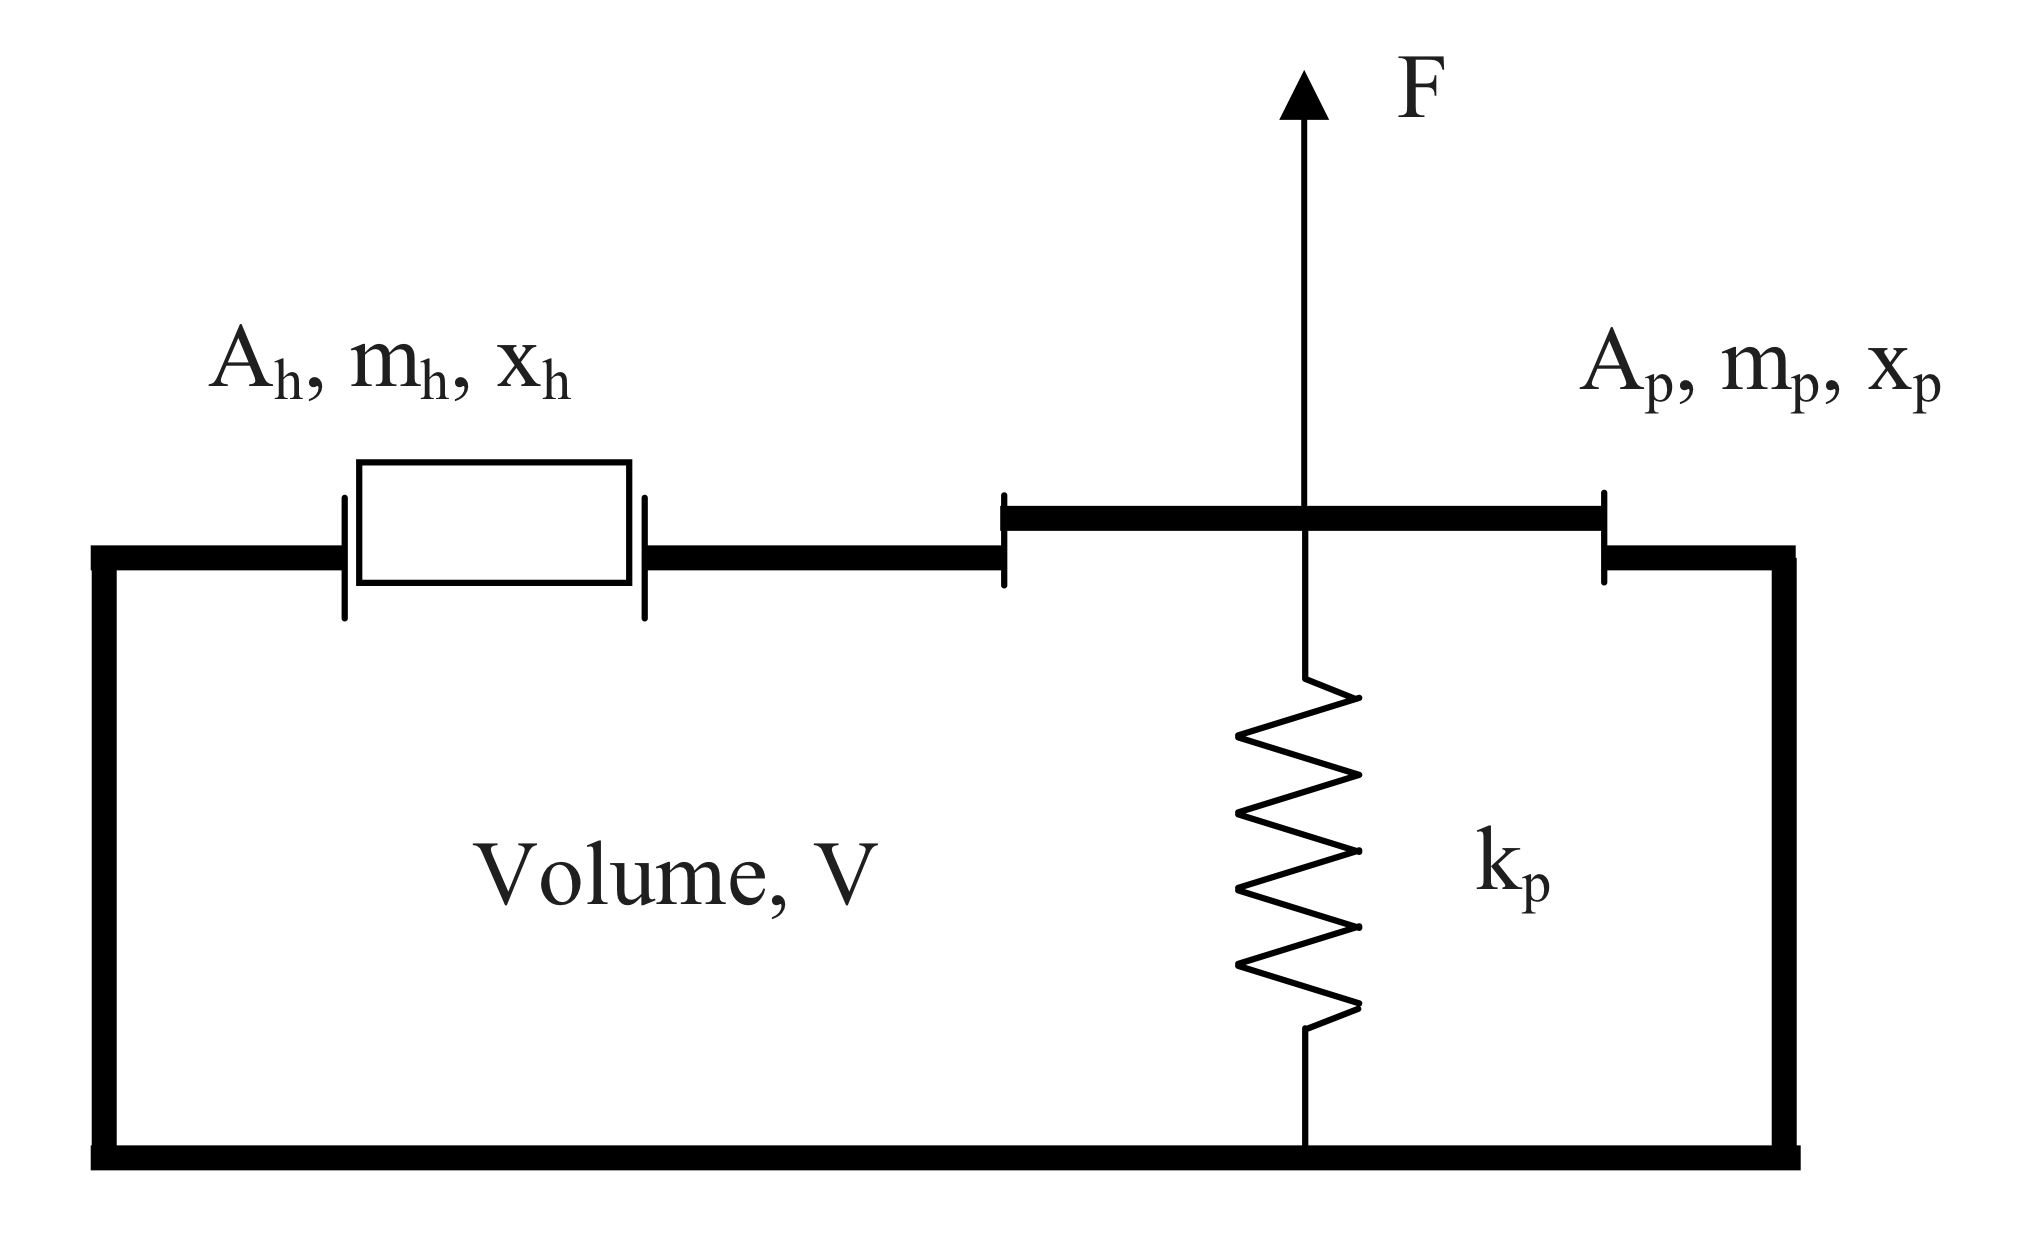
\includegraphics[width=0.4\textwidth]{images/french2008-two-mass-model.png}
        \caption{Two-mass model of the low-frequency behavior of the guitar. The soundboard and guitar cavity are replaced by coupled oscillators.  Reprinted from  French, R. (2008). Engineering the Guitar: Theory and Practice. Springer US.}
        \label{fig:two-mass-model}
    \end{center}
\end{figure}
\begin{figure}[ht]
    \begin{center}
        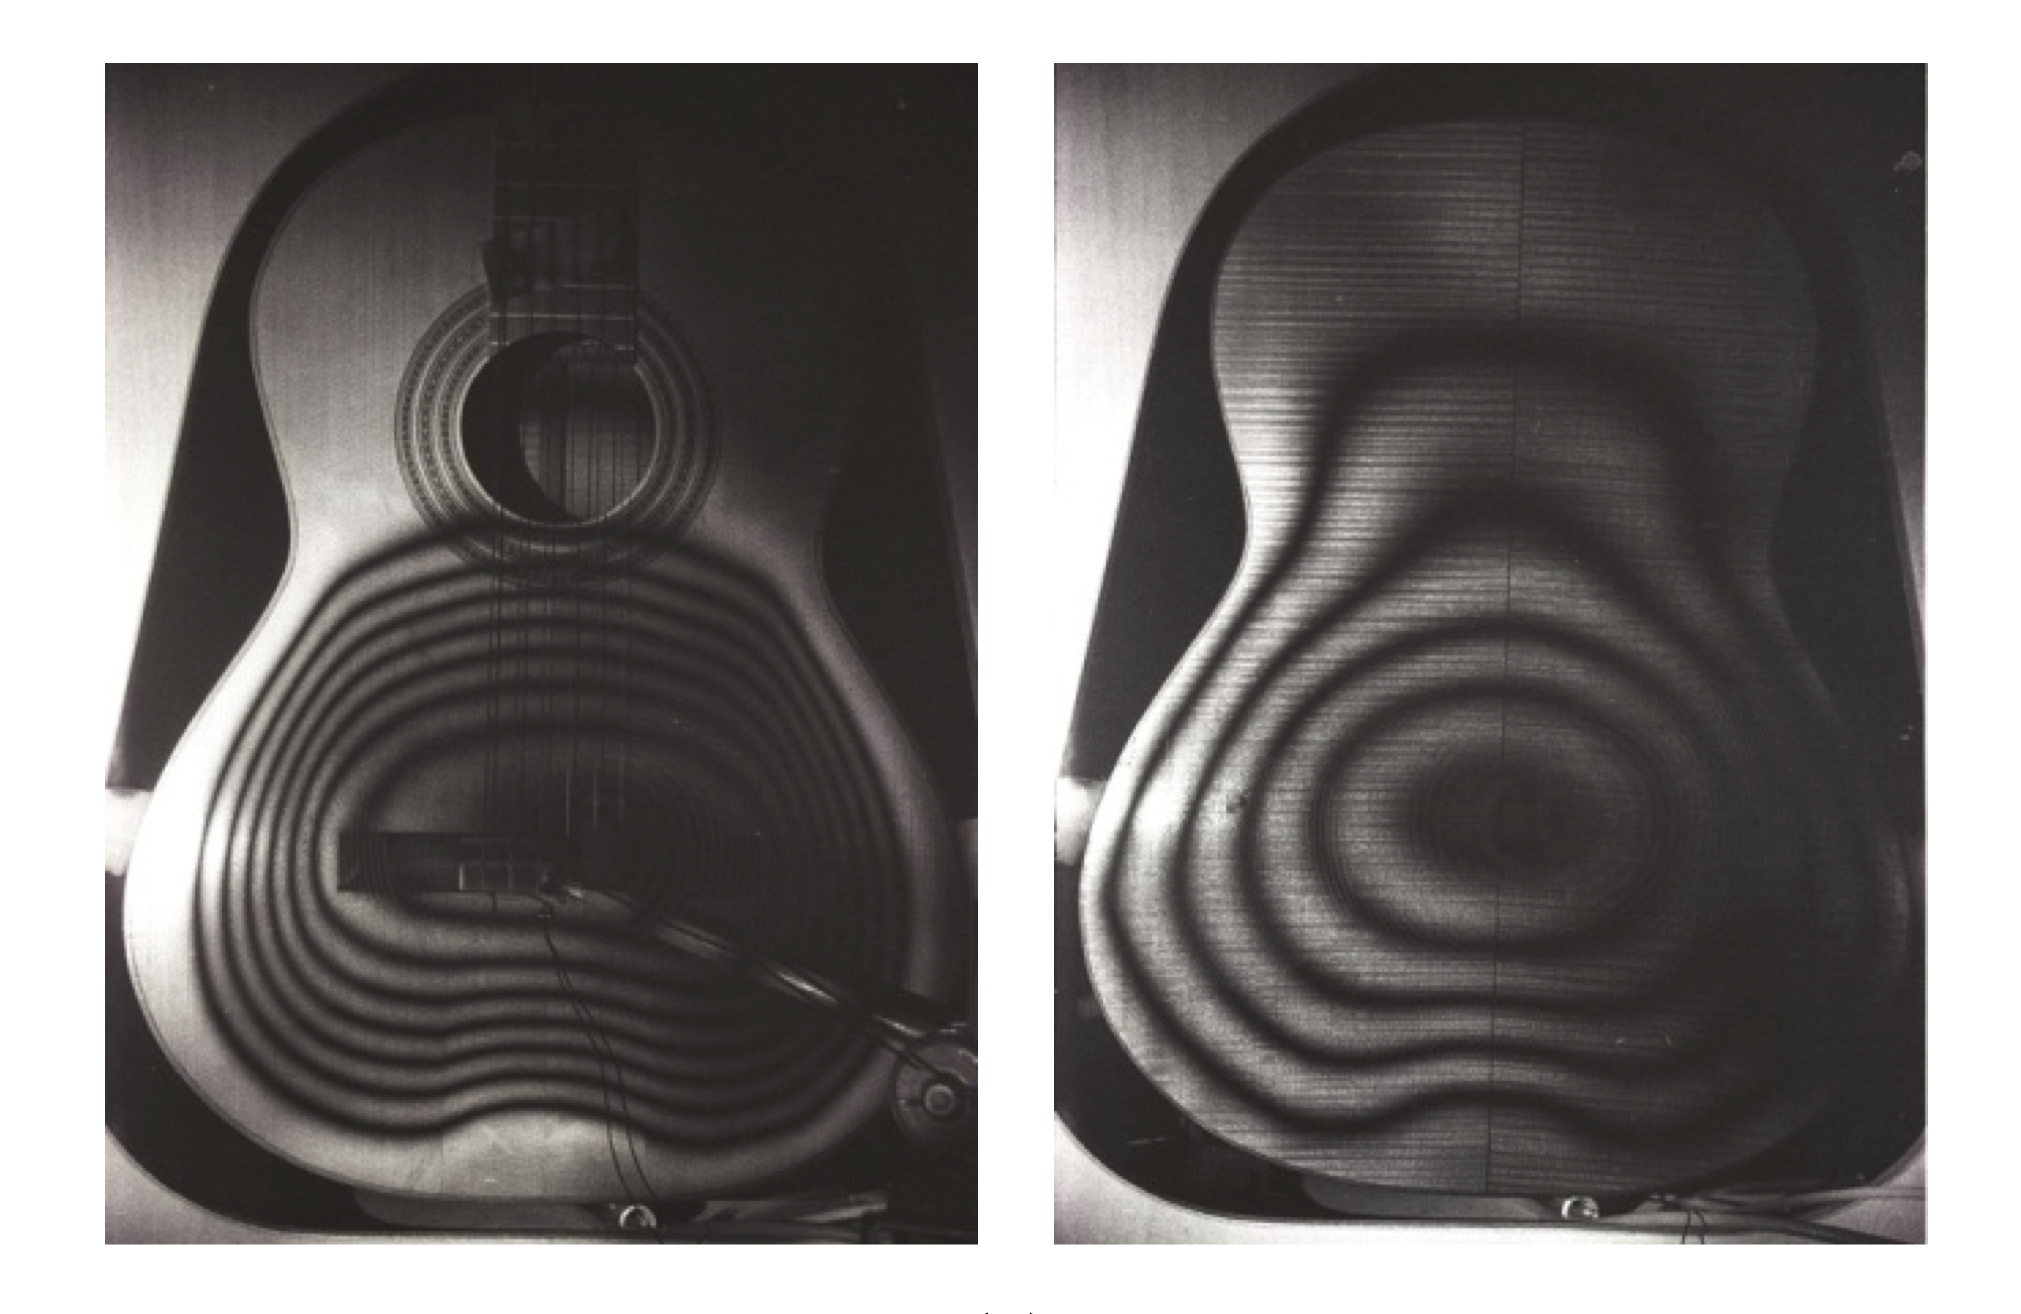
\includegraphics[width=0.4\textwidth]{images/richardson2012-fundamental-modes-holography.png}
        \caption{Visualization of the fundamental resonance of a classical guitar using holographic interferometry. On left is the top plate, on right is the back. Reprinted from Richardson, B., Johnson, H., Joslin, A., and Perry, I. (2012). The three-mass model for the classical guitar revisited. In d’Acoustique, S. F., Acoustics 2012, Nantes, France.}
        \label{fig:holography-fundamental-mode}
    \end{center}
\end{figure}
As a justification of this model, Figure \ref{fig:holography-fundamental-mode} shows a visualization of the fundamental mode of the top and back plates made using holographic interferometry. The fundamental mode of the top plate is a symmetric mode in the lower bout with no interior node lines, similar to the symmetric modes of a fixed-rim circular membrane. For wavelengths significantly larger than the dimensions of the source, the radiated pressure field depends primarily on the volume displacement rather than the shape of the resonator, and substitution with a simple piston of equivalent volume displacement is justified \cite{kinsler2000fundamentals}. The mass and equivalent area of the piston are smaller than those of the real soundboard, and are considered experimental parameters to be determined by loading the plate with a known mass and observing the resulting shift in natural frequency.

Newton's second law reads:
\begin{align*}
m_p \ddot{x}_p & = & F - (k_p + \mu A_p ^2) x_p - R_p \dot{x}_p - \mu A_h A_p x_h \\
m_h \ddot{x}_h & = & - \mu A^2 x_h - R_h \dot{x}_h - \mu A_h A_p x_p
\end{align*}

where the physical parameters are given in Figure \ref{fig:two-mass-model}, $F$ is a driving force applied to the bridge (strings), $R_p$ and $R_h$ are damping, and $\mu = c^2 \rho / V$ is a proportionality constant between changes in volume and changes in pressure. Two resonances of the coupled system are determined by moving to frequency space and solving for the eigenvalues, the lower of which ($f_-$) is a mode in which the air piston moves in phase with the backside of the top plate and the higher ($f_+$) corresponding with out-of-phase motion.

Figure \ref{fig:experimental-tuning-two-mass} shows the careful experimental process of tuning such a model. Adding mass to the top plate (2 in the figure) actually causes a shift in both $f_-$ and $f_+$ but causes no shift in the intermediate anti-resonance of top plate mobility. The anti-resonance is changed when the soundhole is extended (3) or covered (4), so it is sensitive to the Helmholtz resonance but not the top plate resonance. The frequency of the anti-resonance is therefore representative of the uncoupled Helmholtz resonance, $f_h$, and can be experimentally determined for a given instrument. Similarly, covering the soundhole leaves a single resonance which is characteristic of the top plate and closed cavity uncoupled from the Helmholtz resonator, $f_p$.

A general system of $n$ coupled oscillators can be described by
\begin{equation*}
\mathbf{M}\mathbf{\ddot{x}} + \mathbf{R}\mathbf{\dot{x}} + \mathbf{K} \mathbf{x} = \mathbf{F}
\end{equation*}
where $\mathbf{x}$ is a vector of length n describing the positions of all oscillators, $\mathbf{M}$, $\mathbf{K}$, and $\mathbf{R}$ are the mass, stiffness, and damping matrices, and $\mathbf{F}$ is any external driving force. Assuming a harmonic response and driving force, the normal modes are determined by the eigenvalue relationship $(\mathbf{K} + i \omega \mathbf{R} - \omega ^2 \mathbf{M})\mathbf{a} = 0$ where $\mathbf{a}$ is a normal mode of the coupled system with frequency $\omega$. The trace of $(\mathbf{K} + i \omega \mathbf{R} - \omega ^2 \mathbf{M})$ simply gives the sum of squares of the natural frequencies of the individual \emph{uncoupled} oscillators, and the trace of a diagonalizable matrix is always the sum of its eigenvalues. The useful result is that $\sum (\omega_i)^2$ is the same for the normal modes of a coupled system as it is for the individual resonances of the uncoupled oscillators. This relationship can be used to constrain effective parameters of the coupled system, such as $f_p$, in terms of uncoupled parameters which are easier to calculate. It is also a useful sanity check of the modes predicted by a lumped parameter model.

Here, the fundamental top plate mode can be determined by measuring $f_-$, $f_+$, and $f_h$ (which are not sensitive to mass loading on the top plate due to experimental equipment) and applying $f_+ ^2 + f_- ^2 = f_p ^2 + f_h ^2$. Similarly, $f_p$ can be related to the top plate mass and effective piston areas by considering the resonance of the closed cavity $2 \pi f_p = [(k_p + \mu A_p ^2)/m_p]^{1/2}$ compared to the resonance of the cavity with no coupling $2 \pi f_a = (\mu A_p ^2 / m_p) ^{1/2}$. The top plate resonance in the absence of any cavity $f_{p, 0}$ is then given by $f_p ^2 = f_{p, 0} ^2 + f_a ^2$. By varying the top plate mass and observing the change in $f_p$ determines equivalent top plate mass $m_p$, after which $f_{p, 0}$ gives the top plate stiffness.

\begin{figure}[ht]
    \centering
        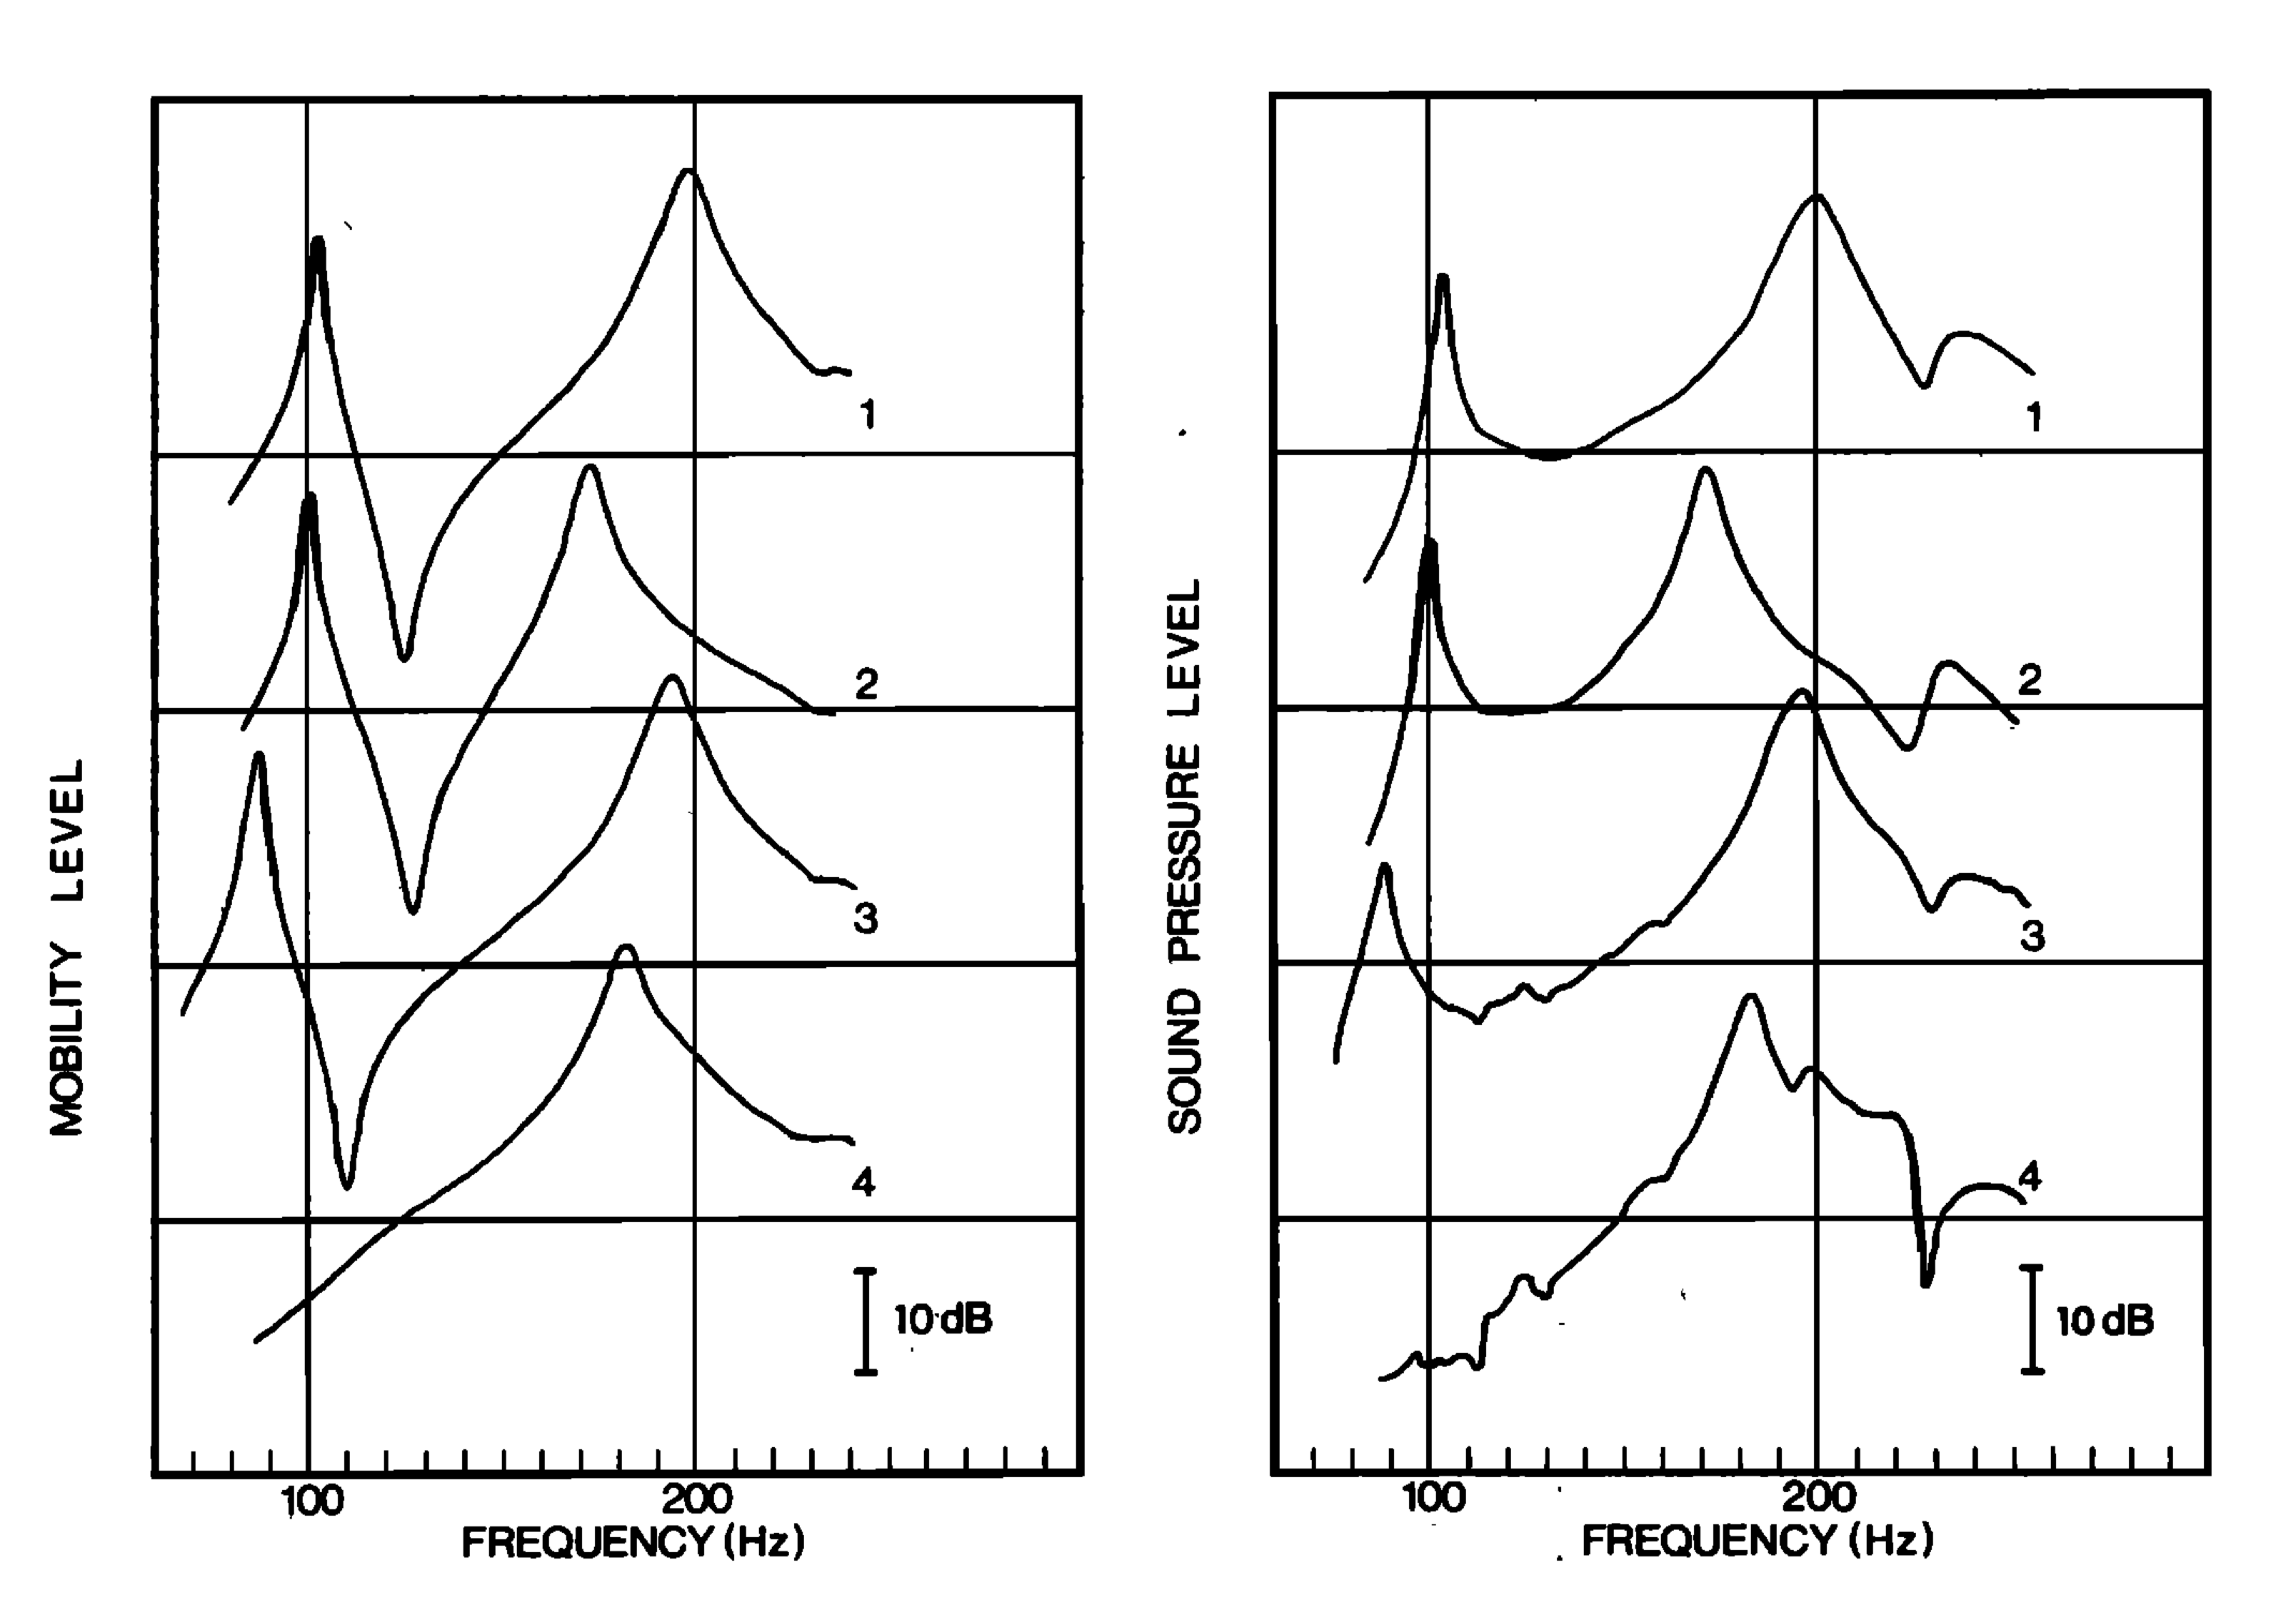
\includegraphics[width=0.4\textwidth]{images/christensen1980-two-mass-coupling-experiment.png}
        \caption{Effects of specific modifications to the top plate and Helmholtz resonances on mobility level of top plate (left) and sound pressure level 2m above the center of the top plate. Modifications to the instrument are (1) normal guitar; (2) mass loading of 39.3g to top plate; (3) 3 cm cylindrical "collar" inserted into soundhole; (4) soundhole plugged with wooden disk.  Reprinted from  Christensen, O. and Vistisen, B. B. (1980). Simple model for low-frequency guitar function. The Journal of the Acoustical Society of America, 68(3):758–766.}
        \label{fig:experimental-tuning-two-mass}
\end{figure}

\begin{figure}[ht]
    \centering
        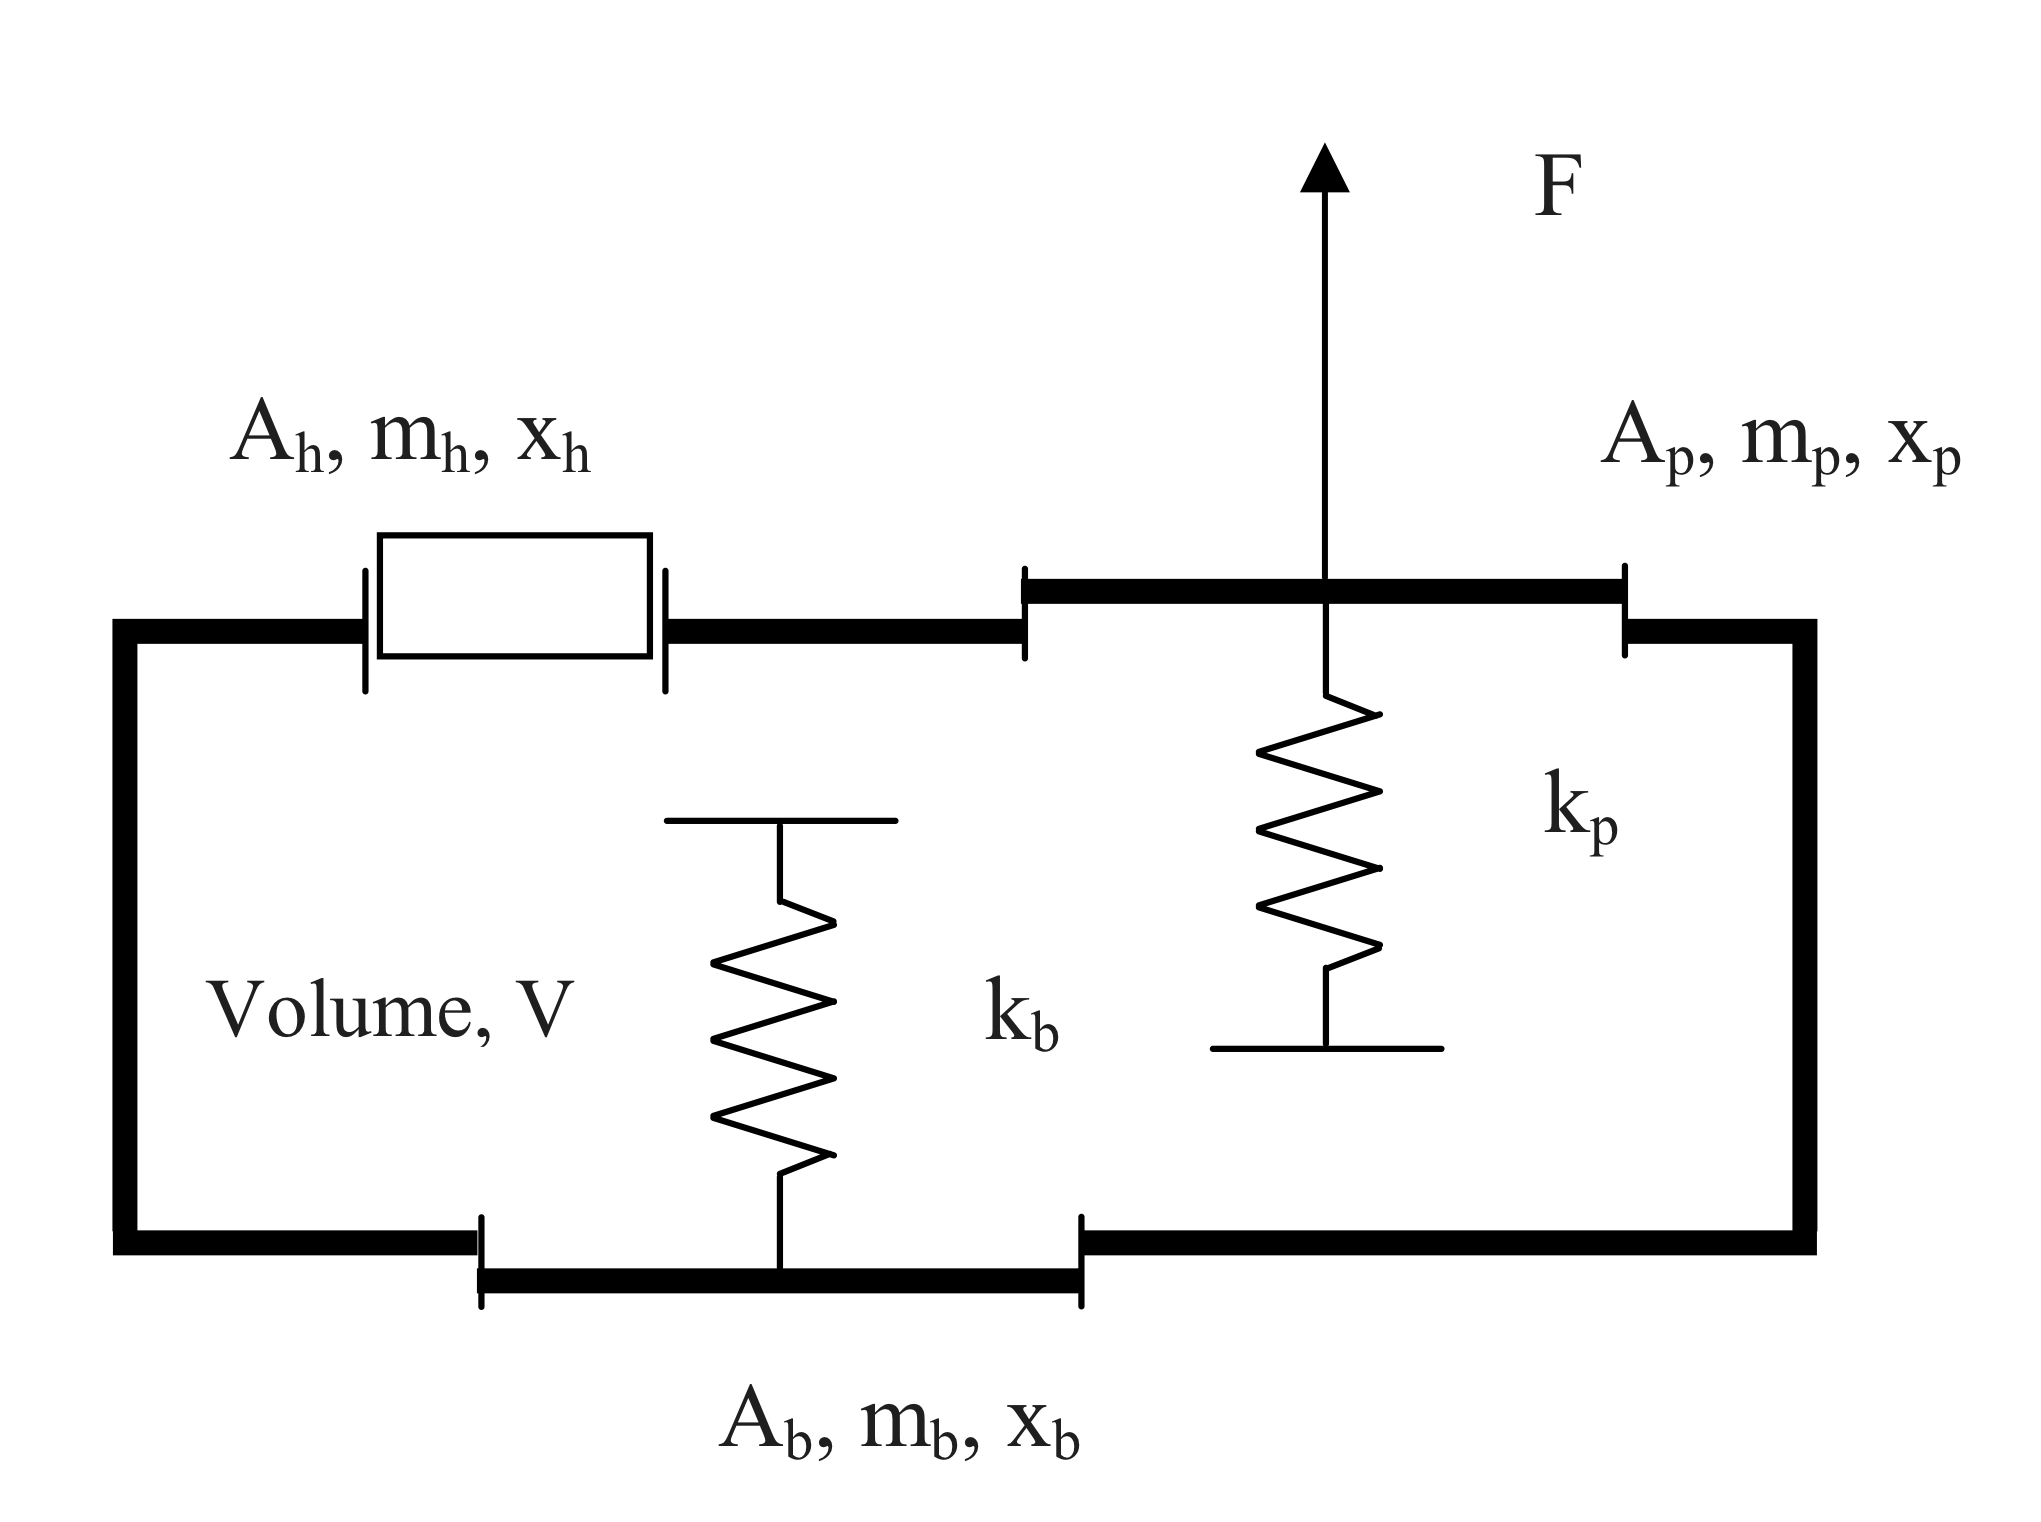
\includegraphics[width=0.4\textwidth]{images/french2008-three-mass-model.png}
        \caption{Three degree of freedom model including the back of the instrument as a third coupled oscillator.  Reprinted from  French, R. (2008). Engineering the Guitar: Theory and Practice. Springer US.}
        \label{fig:three-mass-model}
\end{figure}

Typical real guitars display a third resonance in the range 90-240Hz.\cite{lee2016:doi:10.1155/2016/6084230} The two-mass model can be readily extended by treating the back of the guitar as analogous to the soundboard, as shown in Figure \ref{fig:three-mass-model}. The equations of motion are now \cite{french2008engineering}
\begin{align*}
\begin{bmatrix}
m_p & 0 & 0 \\
0 & m_h & 0 \\
0 & 0 & m_b
\end{bmatrix}
\begin{bmatrix}
\ddot{x_p} \\
\ddot{x_h} \\
\ddot{x_b}
\end{bmatrix} +
\begin{bmatrix}
R_p & 0 & 0 \\
0 & R_h & 0 \\
0 & 0 & R_b
\end{bmatrix}
\begin{bmatrix}
\dot{x_p} \\
\dot{x_h} \\
\dot{x_b}
\end{bmatrix} & \\
+ 
\begin{bmatrix}
k_p + \mu A_p ^2 & \mu A_h A_p & \mu A_p A_b \\
\mu A_h A_p & \mu A_h ^2 & \mu A_b A_h \\
\mu A_p A_b & \mu A_b A_h & k_b + \mu A_b ^2
\end{bmatrix}
\begin{bmatrix}
x_p \\
x_h \\
x_b
\end{bmatrix} & = 
\begin{bmatrix}
F \\
0 \\
0
\end{bmatrix}
\end{align*}

The third degree of freedom adds a third normal mode and a third peak to the resulting frequency response function. The three fundamental modes now present are: a "breathing" mode in which the top and back plates move out of phase and the air piston moves out of phase with the top plate, an "anti-breathing" mode in which the air piston instead moves in phase with the top plate, and a "bending" mode in which the top and back plates are in phase. When compared with the next 20 higher-order modes, these three fundamental modes have the major controlling influence on the playing qualities of the guitar.\cite{richardson:hal-00811279}

By adding an additional degree of freedom to the model, an important fundamental mode of the instrument is recovered, but at a cost in complexity. There are now more unknown effective parameters of the equivalent oscillators than there are fundamental frequencies. Various modifications can be made to over-constrain the model for a given instrument and ensure physically meaningful results. For example, covering the soundhole will cause the Helmholtz resonance to disappear, shifting the other frequencies slightly. Adding weights to both the top and back of the instrument allow for a variety of effective piston masses. Minimizing the errors between the measured and predicted normal modes results in a tuned model.\cite{french2008engineering}

\begin{figure}[ht]
    \begin{center}
        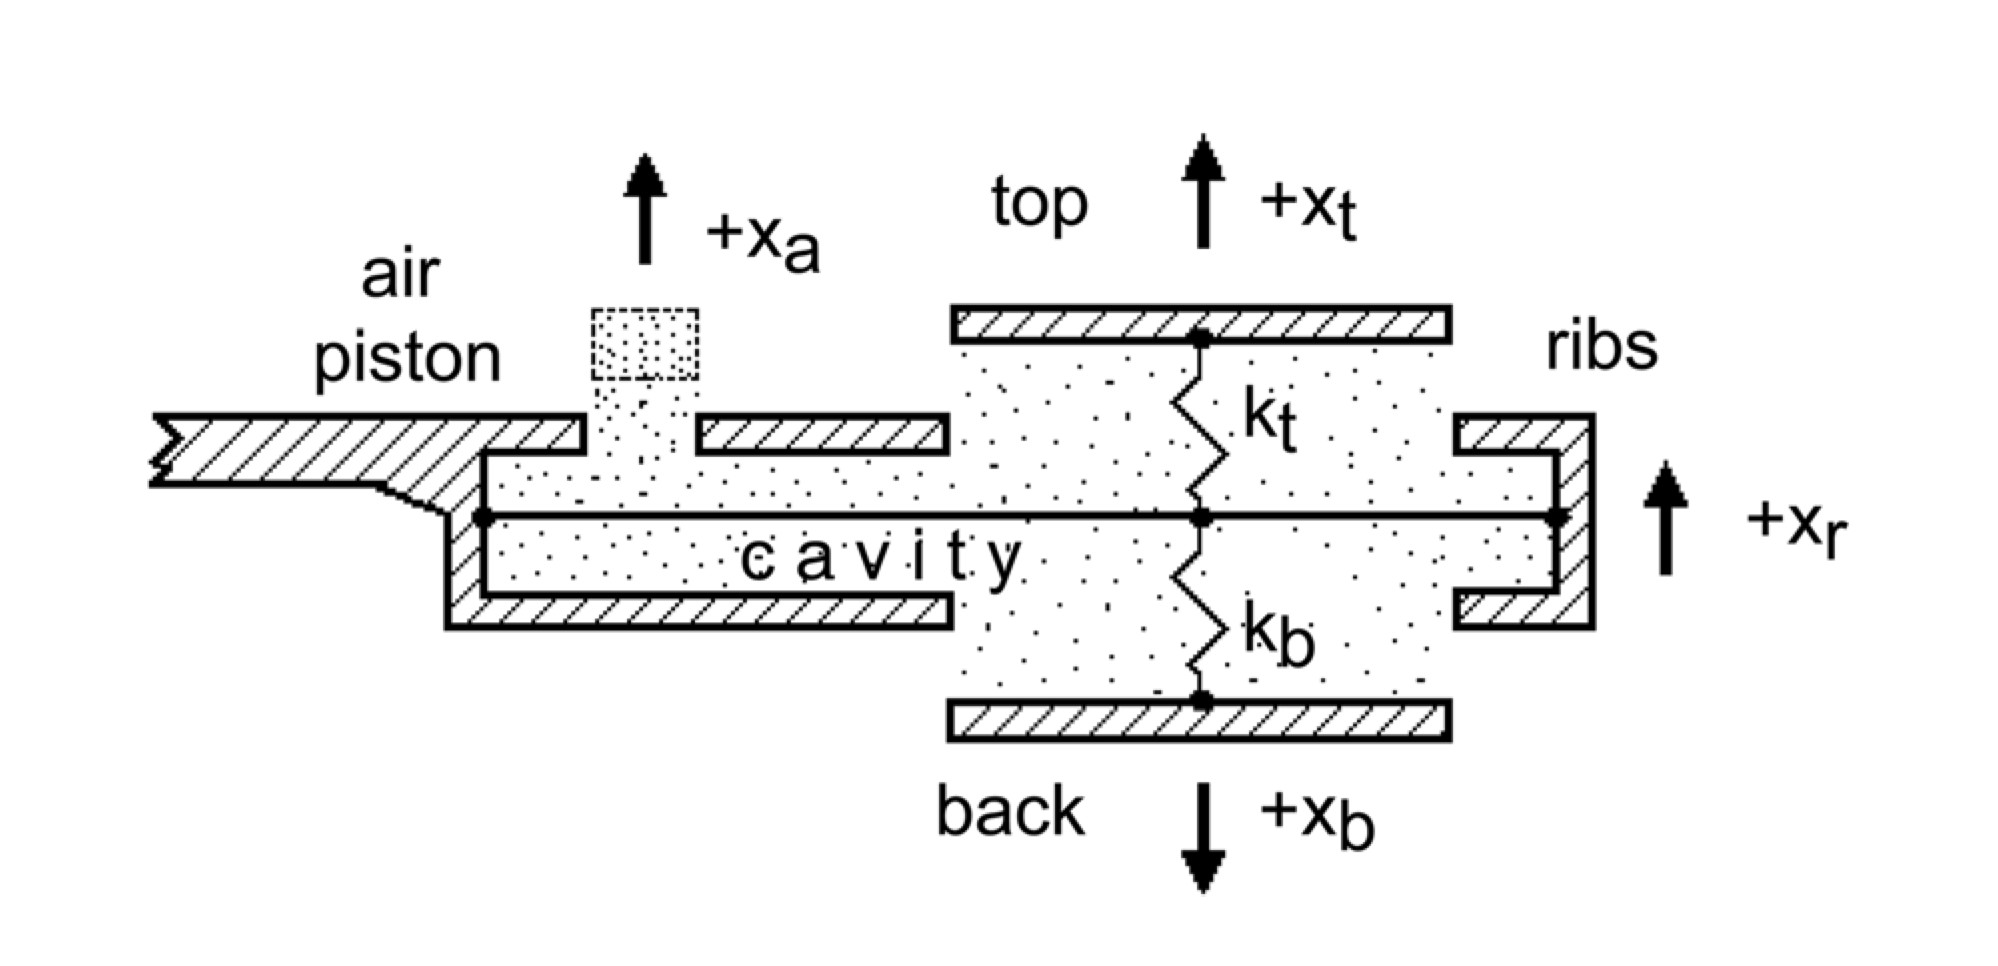
\includegraphics[width=0.4\textwidth]{images/popp2012-four-mass-model.png}
        \caption{Addition of the ribs (neck and sides) of the guitar as a fourth oscillator. Reprinted from Popp, J. E. (2012). Four mass coupled oscillator guitar model. The Journal of the Acoustical Society of America, 131(1).}
        \label{fig:four-mass-model}
    \end{center}
\end{figure}

Thus far we have assumed that the sides and neck of the guitar are stationary, but this is not a valid assumption under normal playing conditions. Popp\cite{PoppJohnE2012Fmco} explores the result of adding an additional oscillator in the form of the sides and neck, termed "ribs" (see Figure \ref{fig:four-mass-model}). The additional degree of freedom does not result in an additional eigenmode. Rather, it amounts to a modification of the boundary conditions of the three-mass model, by assigning the ribs a non-infinite mass rather than treating the sides as clamped. The result is a shifting in the frequency of the "bending" mode dependent on the rib mass. The other two low-frequency modes (breathing and anti-breathing) are largely unaffected by the rib mass because they involve in-phase movement towards and away from the center of mass, causing very little recoil of the ribs.

In the case of a modelled Martin D28 guitar, if rib mass is varied through a realistic range around 0.35kg the frequency of the bending mode drops and approaches that of the anti-breathing mode. When the two coincide, the two modes are replaced by a new mode in which the top plate and air piston move in phase with each other, and the back and ribs move in the direction opposite to the top and air piston. This behavior was not present in a Kohno classical guitar modeled in the same way, presumably because unlike the other guitars studied, the D28 had a much lighter and softer back than top, and because it had a bending mode near the frequency of its anti-breathing mode. For a typical classical guitar, the effect of the rib mass is largely insignificant, and according to Richardson adding more than three oscillators is an unnecessary complication for this method of low-frequency modelling.\cite{richardson:hal-00811279}

The finite-element method is an excellent complementary technique to this type of lumped parameter modal analysis. While the latter technique can reveal a great deal about the sound produced by the complete instrument, it replaces the physical parameters of the real guitar with effective values and in doing so sacrifices the ability to directly describe the influences of various parts of the construction process on the final sound. Elejabarrieta et. al gives an example of using the finite-element method to gain further insight into the results of analytical models.\cite{elejabarrieta2002:doi:10.1121/1.1470163} A high-accuracy numerical model of a real guitar resonance box was constructed additively, starting with isolated front and back plates, followed by the sides and blocks, then the air within the guitar body.  The finite element model of the resonance box was carried out using ABAQUS software, and the resulting coupled mode analysis performed using SYSNOISE software. The resolution of the model permitted modal analysis of frequencies up to 500Hz, so was limited to the low-frequency regime of the guitar. Figure \ref{fig:finiteelement} shows the mesh used, including sheet elements for the ribs and brick elements for the other various pieces, blocks, and edges.

\begin{figure}[ht]
    \begin{center}
        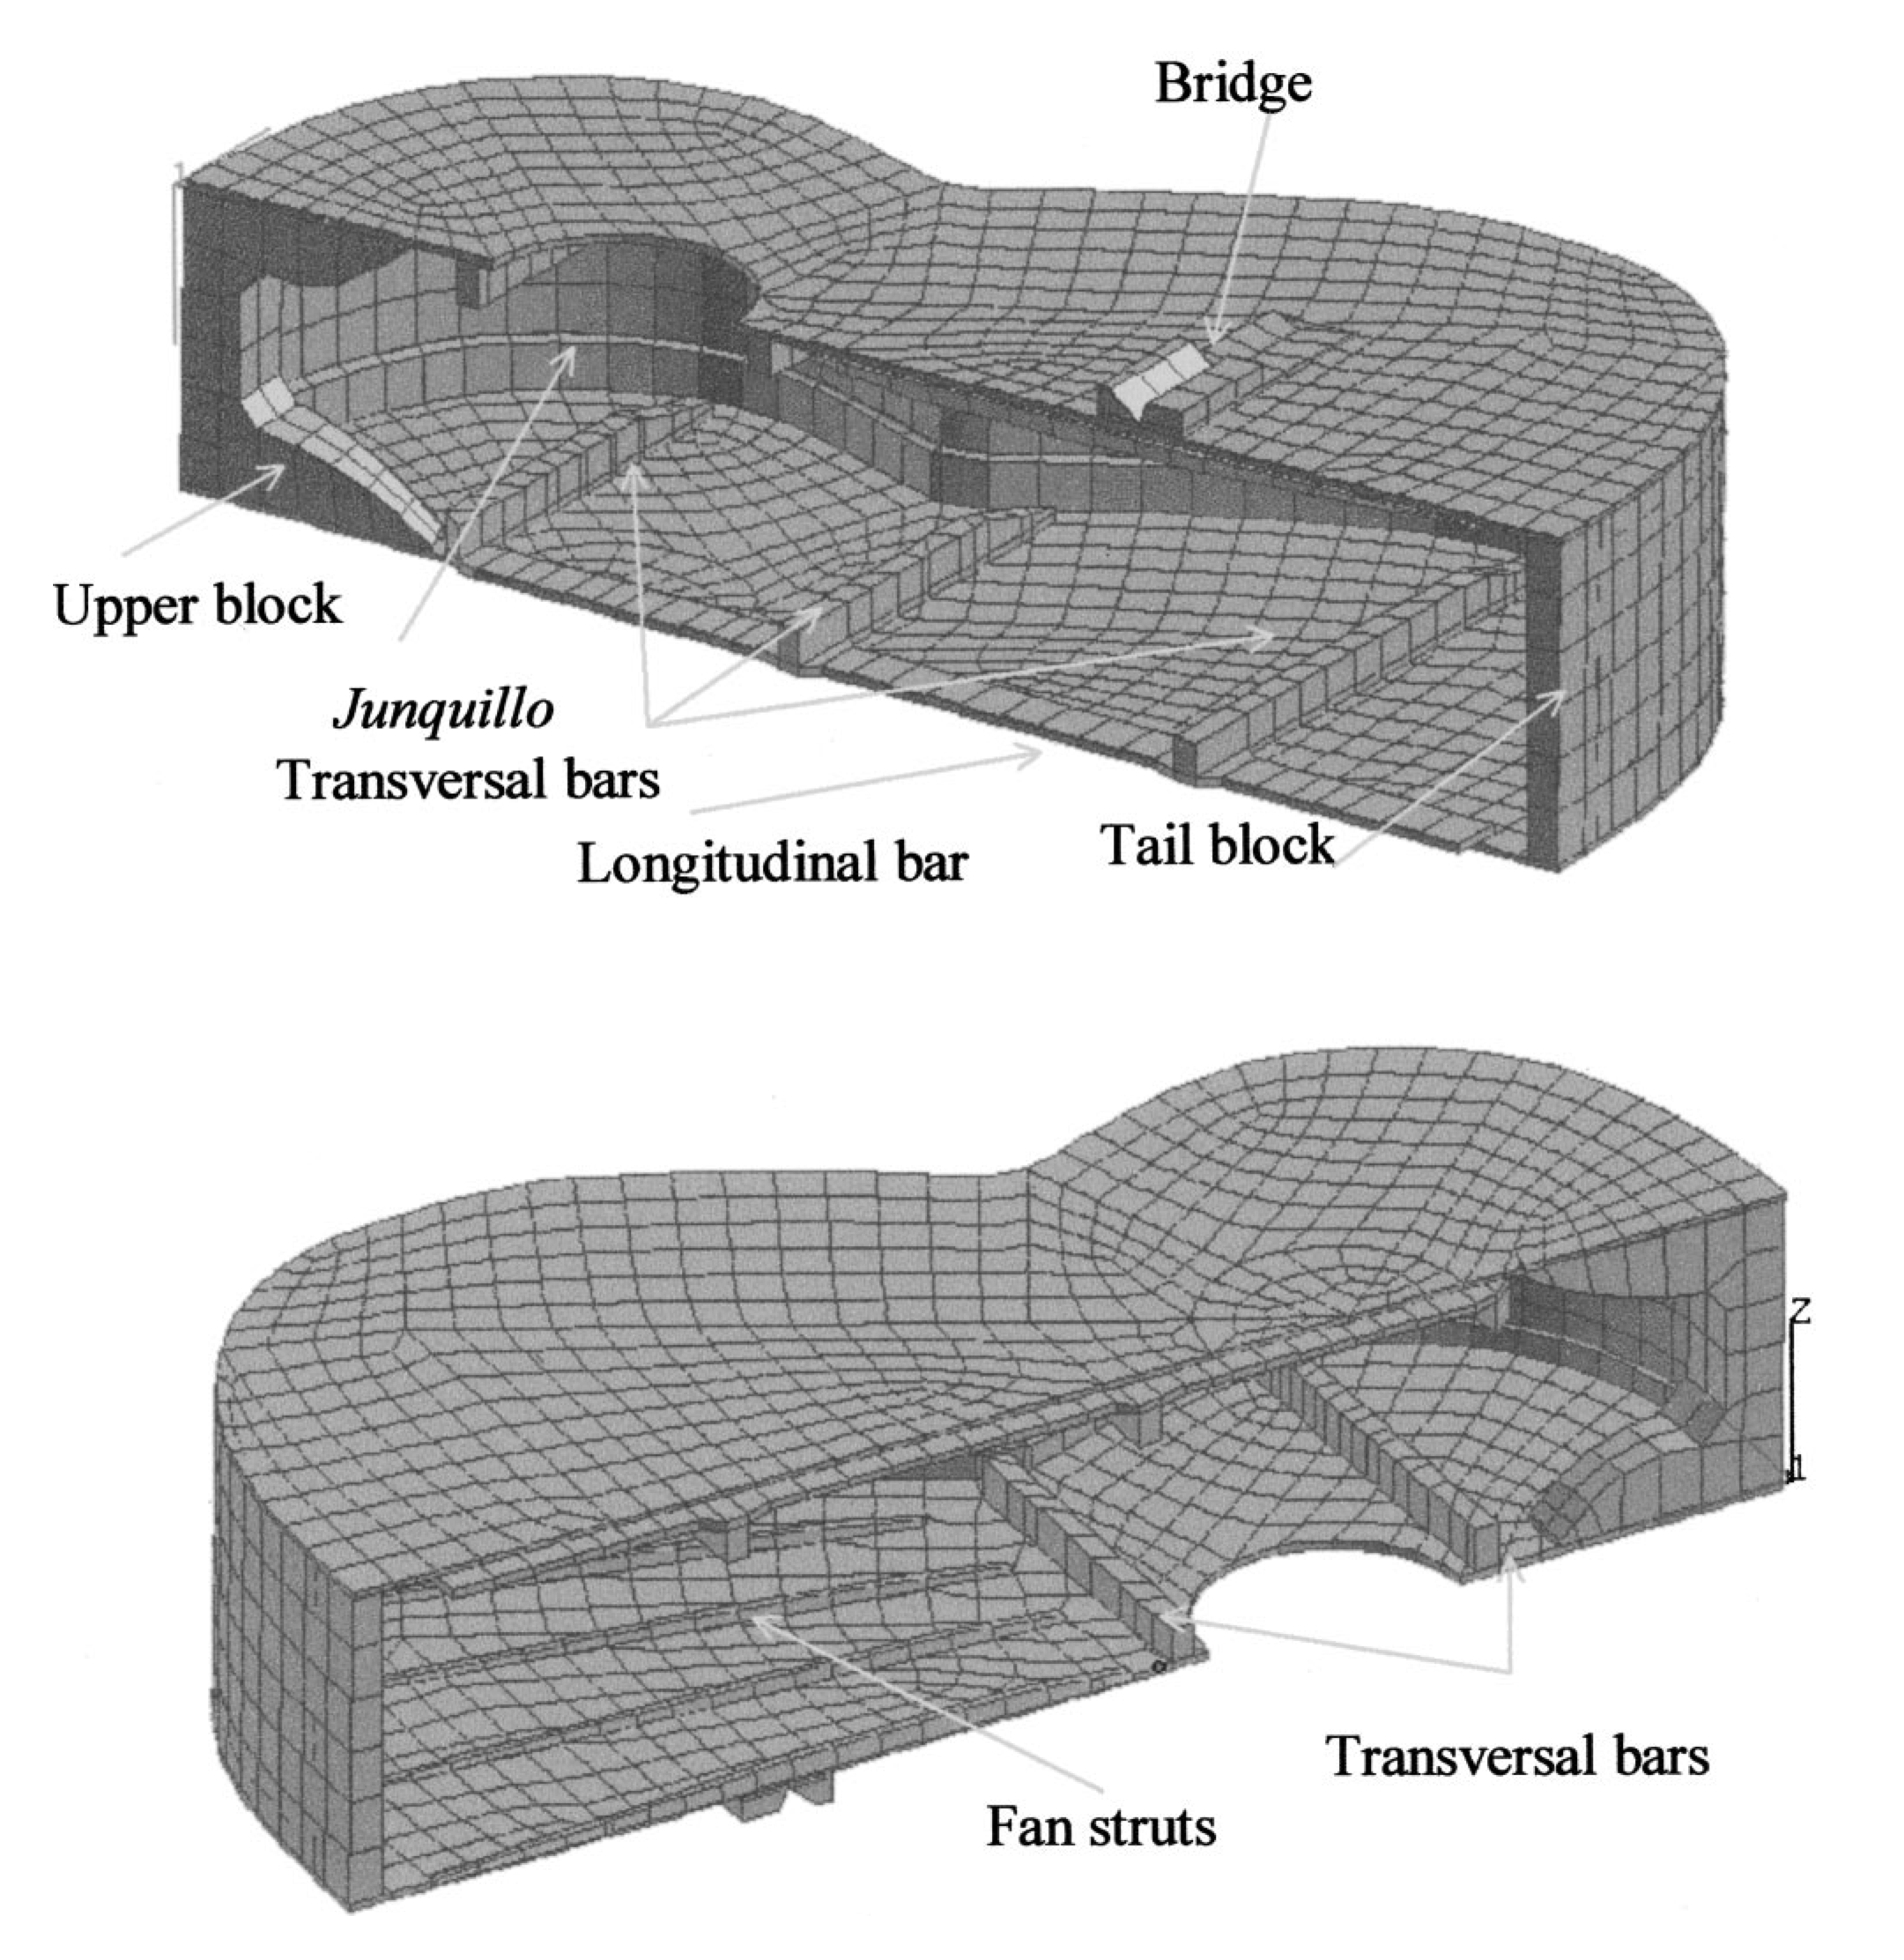
\includegraphics[width=0.4\textwidth]{images/elejabarrieta-fe-model.png}
        \caption{Finite element mesh used in simulations of a guitar resonance box. Reprinted from Elejabarrieta, M. J., Ezcurra, A., and Santamara, C. (2002b). Coupled modes of the resonance box of the guitar. The Journal of the Acoustical Society of America, 111(5):2283–2292.}
        \label{fig:finiteelement}
    \end{center}
\end{figure}

The benefit of developing the model progressively is the ability to directly establish the influence of each component of the body of the guitar on the real action of the resonance box. Comparison of the modal analysis of the "empty" (airless) resonance box with and without the ribs confirms that there is no coupling is possible between the soundboard and the back plate without the presence of air. The assembly process only affects the natural frequencies of modes presenting vibration in the upper region of the body near the top block, so the behavior of the assembled body can be predicted from the dynamics of the individual components. A preliminary finite element model assuming a rigid cavity determined the modes of the air within the body cavity \cite{elejabarrieta2002:aircavitymodes}, with the lowest and most important being the Helmholtz-like mode. Due to the frequencies involved and the non-constant volume of the guitar body, the fundamental mode does not have uniform pressure throughout and is not a pure Helmholtz mode.

Adding air within the guitar body to the model results in the coupling between the top and bottom plates. The calculated coupled modes and their natural frequencies were shown to be in good agreement with those measured from a real guitar resonance box. Expanding the modes of the fully coupled system in terms of contributions from the modes of the individual components of the guitar allows for calculation of participation factors from each of the uncoupled modes. As an example, the fundamental "breathing" mode is a coupling of the fundamental modes of the top and bottom plate moving in opposite directions while the upper portion of the soundboard remains motionless. For the particular instrument modelled, the fundamental modes of the top and bottom plate  interact with participation factors 70\% and 26\% respectively. The coupling between the top and back plates is expanded in terms of the modes of the air within the guitar body, with the Helmholtz mode accounting for 97\%.  We can conclude that this mode is sensitive to any changes in the wood or struts which would alter the fundamental mode of the soundboard, and also to any changes in the sound hole and guitar volume which would affect the Helmholtz mode. Similar insights can be gained for the other coupled modes.

Lumped parameter analytic models of guitar function give a good dynamic description for low frequencies, where the majority of acoustical energy is radiated. It should not be forgotten that the quality of an instrument is not determined only by its low-frequency response. The human range of hearing can extend to 20 kHz, and a complete characterization with the ability to discern a high-quality instrument from lower quality ones should extend the bandwidth under investigation up to at least 5 kHz\cite{CzajkowskaMarzena2012Aocg}. While it is possible to extend the lumped parameter model to an arbitrary number of elements, the underlying assumptions and simplicity break down at higher frequencies, requiring detailed finite-element and boundary-element models are required to complete the picture.


\setstretch{1.0}
\nocite{*}
\bibliographystyle{apalike}
\bibliography{paper}% Produces the bibliography via BibTeX.

\end{document}
%
% ****** End of file apssamp.tex ******
